\documentclass{acm_proc_article-sp}

\usepackage[utf8]{inputenc}
\usepackage{caption,subcaption}
\captionsetup{labelfont=bf}
\usepackage[]{microtype}

% for proper backquote
\usepackage{upquote}

% URLs
\usepackage{url}
\usepackage[hidelinks]{hyperref}

% color

\usepackage{color}
\usepackage{xcolor}

% listings
\usepackage{listings}
\lstset{
  numbers=left,
  numberstyle=\tiny,
  basicstyle=\ttfamily\small,
  belowcaptionskip=0em,
  aboveskip=1.5em,
  belowskip=0em,
  mathescape=true,
  captionpos=b,
  rulecolor=\color{black},
  prebreak = \raisebox{0ex}[0ex][0ex]{\ensuremath{\hookleftarrow}},
  frame=b,
  xleftmargin=2em,
  framexleftmargin=2em,
  xrightmargin=0pt,
  resetmargins=true,
  framerule=1pt
}

%% Side-by-side listings

\usepackage{subfig}
\usepackage{caption}
\captionsetup{format=hang}

\usepackage{subcaption}
\usepackage{floatrow}

\makeatletter
\newbox\sf@box
\newenvironment{sublisting}[2][]{%
\def\sf@one{#1}%
\def\sf@two{#2}%
\setbox\sf@box\hbox
\bgroup
}{%
\egroup
\ifx\@empty\sf@two\@empty\relax
\def\sf@two{\@empty}
\fi
\ifx\@empty\sf@one\@empty\relax
\subfloat[\sf@two]{\box\sf@box}%
\else
\subfloat[\sf@one][\sf@two]{\box\sf@box}%
\fi
}
\makeatother

\newfloat{mylisting}{htbp}{lom}
\restylefloat*{mylisting}
\floatstyle{plain}
\floatname{mylisting}{Listing}
\captionsetup[mylisting]{position=bottom}
\floatsetup[mylisting]{}
\newsubfloat[position=bottom]{mylisting}
\captionsetup[subfloat]{lomdepth=2}
% use listing counter
\makeatletter
\AtBeginDocument{\let\c@mylisting\c@lstlisting}
\makeatother

%% Quotation with signature

\usepackage{quoting}
\quotingsetup{vskip=0pt}

\def\signed #1{{\leavevmode\unskip\nobreak\hfil\penalty50\hskip2em
  \hbox{}\nobreak\hfil(#1)%
  \parfillskip=0pt \finalhyphendemerits=0 \endgraf}}

\newsavebox\mybox
\newenvironment{aquote}[1]
  {\savebox\mybox{#1}\begin{quoting}}
  {\signed{\usebox\mybox}\end{quoting}}


%% tikz

\usepackage{tikz}
\usetikzlibrary{positioning,shapes,arrows,calc}
\newcommand*{\h}{\hspace{5pt}}% for indentation
\newcommand*{\hh}{\h\h}% double indentation
\tikzstyle{object}=[rectangle, rectangle split, draw=black,
  text=black, minimum width=2cm,
  rectangle split part align={center,left,left},
  rectangle split part fill={gray!20,white,white}]
\tikzstyle{every text node part}=[align=center]
\tikzstyle{every node}=[font=\small\sffamily]
\tikzstyle{line} = [draw, thick, -latex']
\newcommand{\renvoi}[3][pos=0.5]{
\path (#2) -- (#3)coordinate[#1](mm);
\draw[line] (#2) -| (mm) |- (#3);
}


%%%% Document

\begin{document}

\title{Ralph - A Dylan dialect that compiles to JavaScript}

\numberofauthors{1}

\author{
  \alignauthor
  Bastian Mueller\\
  IT University of Copenhagen, Denmark\\
  \email{\href{mailto:bmue@itu.dk}{bmue@itu.dk}}
}

\maketitle

\begin{abstract}
We present the object-centered dynamic functional programming language
Ralph, which is inspired by Lisp. Ralph supports an extended subset of
Dylan's features (the intermediate Dylan standard with a prefix
syntax) and compiles to JavaScript. The Ralph compiler produces more
efficient JavaScript code than similar compilers translating Lisp-like
languages due to some trade-offs and utilization of an intermediate
representation based on the Administrative normal form. We discuss the
Ralph language, its mechanics, implementation of its features in
JavaScript, and its multi-pass compilation approach.
\end{abstract}

\section{Introduction}
Ralph\footnote{Available at \url{https://github.com/turbolent/ralph}}
is a programming language that targets JavaScript, more specifically
its subset ECMAScript \cite{ecma262}. Ralph is a Lisp dialect mainly
inspired by Dylan \cite{shalit1996dylan} as specified in the first
edition of its manual \cite{shalit1992dylan} (from here on referred to
as ``early specification''). Dylan is based on Scheme, Common Lisp,
and Smalltalk. Like Scheme and unlike Common Lisp, Dylan has a single
namespace for functions and variables. The object system is derived
from the Common Lisp Object System (CLOS), featuring multiple
inheritance and generic functions performing multiple dispatch.

Dylan was invented by Apple and its original code-name was ``Ralph''.
The same name was chosen for the new language to imply the effort of a
partial reimplementation. Unlike the final and standardized version of
Dylan which features an ALGOL-like syntax, this early version still
used a syntax with prefix notation based on s-expressions
\cite{mccarthy1960}.

Ralph provides many of Dylan's features, special forms, macros, and
functions of the standard library. However, it has a simplified
abstraction for collections, condition system and numerical tower. It
provides a module system, procedural hygienic macros and easy
interoperability with JavaScript. The class-based object system
currently supports single inheritance and single dispatch.

Today it is possible to write rich applications for both desktop and
mobile devices using Web technologies. Modern browsers offer a
number of APIs for this purpose, but JavaScript is the only programming
language able to use them. Besides the usage on the client-side,
JavaScript has also become popular for server-side applications,
through environments such as Node.js. JavaScript execution
environments and their underlying engines have evolved from simple
interpreters to sophisticated virtual machines involving Just-In-Time
emission of native code.

JavaScript is a functional programming language influenced by Scheme
and Self: it supports first-class functions, closures, lexical
scoping, higher-order programming, dynamic typing and prototype based
object-oriented programming.

Because of these features, an increasing number of compilers are
targeting JavaScript, both for existing languages, new languages or
low-level byte-code. For example, the Google Web Toolkit allows
writing applications in Java, Parenscript is a compiler for a subset
of Common Lisp, and ClojureScript is a compiler for a subset of
Clojure. CoffeeScript provides an alternative syntax for JavaScript.
Emscripten is a compiler translating LLVM bytecode to JavaScript.

Ralph was designed for use in application development. It is dynamic
to allow rapid prototyping and development, and has a focus on
expressiveness and efficiency. Much like Dylan, it tries
to bring the advanced features of Lisp to non-Lisp programmers, having
a good trade-off between sophisticated features and
performance. Performance and efficiency are  especially crucial on
mobile devices, which have only limited processing capabilities and
reducing power consumption is important. The compiler of Ralph generates
safe and efficient JavaScript close to hand-written code, due to
trade-offs, utilization of an adequate intermediate representation and
high-level optimizations.

We motivate the problem set by presenting the issues associated with
using JavaScript in Section~\ref{sec:problems}, explaining why it is
desirable to have a higher-level language targeting JavaScript.
Section~\ref{sec:related} is looking into related projects and
compilation approaches. Afterwards we describe our solutions for
several problems in Section~\ref{sec:solution}. We present Ralph's
limitations in Section~\ref{sec:limitations} and describe future work
and conclude in Section~\ref{sec:future}.

\section{Problems with JavaScript}\label{sec:problems}

JavaScript has several problematic features which programmers
constantly have to avoid \cite{crockford2008}. A lexical environment is
only created for functions, \texttt{with} statements and
\texttt{catch} clauses of \texttt{try} statements. Block scope or an
equivalent of a let-expression are not available. Another common
problem is hoisting. Variable and function declarations (but not their
initializers) are moved to the top of their enclosing scope and
default to \texttt{undefined}. An example is shown in
Listing~\ref{lst:hoisting}.

\begin{mylisting}[h]
  \caption{Hoisting of declarations}
  \label{lst:hoisting}
  \vspace{-2em}
  \begin{sublisting}{source}
    \begin{minipage}[b]{.4\textwidth}
      \begin{lstlisting}
function foo() {
    bar();
    var x = 1;
}
      \end{lstlisting}
    \end{minipage}
  \end{sublisting}
  \hfill
  \begin{sublisting}{hoisted}
    \begin{minipage}[b]{.50\textwidth}
      \begin{lstlisting}
var foo;
foo = function () {
    var x;
    bar();
    x = 1;
}
      \end{lstlisting}
    \end{minipage}
  \end{sublisting}
\end{mylisting}
\vspace{-0.5em}

The problematic consequences of these features is illustrated in
the following two programs. In the example shown in
Listing~\ref{lst:hoisting-bug1}, it could be assumed the
conditional in \texttt{bar} fails, due to the initialization of
\texttt{foo} to 1. However, because of hoisting, the conditional
succeeds.

\begin{lstlisting}[caption=Bug caused by hoisting,label=lst:hoisting-bug1]
var foo = 1;
function bar() {
    if (!foo) {
        var foo = 10;
    }
    return foo;
}
bar();  // $\Rightarrow$ 10
\end{lstlisting}

In the second example shown in Listing~\ref{lst:hoisting-bug2}, it
could be assumed the assignment in line 3 would affect the global
variable, but the function declaration is hoisted and a local variable
\texttt{a} is introduced inside function \texttt{b}, even though the
declaration of function \texttt{a} is actually never reached.

\begin{lstlisting}[caption=Hoisting with unreachable code,label=lst:hoisting-bug2]
var a = 1;
function b() {
    a = 10;
    return;
    function a() {}
}
b();
a // $\Rightarrow$ 1
\end{lstlisting}

\texttt{For} loops are not creating new bindings in each iteration.
In combination with closures this leads to another common problem that
is exemplified in Listing~\ref{lst:for-loop}.

\begin{lstlisting}[caption=For loop in connection with closure,label=lst:for-loop]
var fns = [];
for (var i = 0; i < 5; i++) {
  fns.push(function () {
    return i;
  });
}
fns[3]();  // $\Rightarrow$ 5
\end{lstlisting}

The initialization part of the \texttt{for} loop is hoisted and in the
step part, the variable is incremented. The closure added to the array
is containing a reference to the variable, not the value that was
bound when the closure was created.

Another common problem is JavaScript's uncommon semantics of truth and
comparison using the equality operator \texttt{==}, which involves
several coercion rules if its operands are of different types. Some
examples demonstrating the behavior are shown in
Listing~\ref{lst:js-equality}.

\begin{lstlisting}[
    caption=Examples of equality and truth behavior,
    label=lst:js-equality]
'' == '0'              // $\Rightarrow$ false
'' == 0                // $\Rightarrow$ true
'0' == 0               // $\Rightarrow$ true
false == '0'           // $\Rightarrow$ true
' \t\n ' == 0          // $\Rightarrow$ true
' \n ' ? true : false  // $\Rightarrow$ true
\end{lstlisting}

The language is also missing a mechanism to organize code and create
reusable software components that safely interact with each other. For
example, Common Lisp provides packages for this purpose. Dylan
provides modules and libraries. In JavaScript, all scripts loaded into
an environment are evaluated in the global scope, thus leading to
possible interference between programs using identical names.

Even though JavaScript has problems and writing programs
directly is error-prone, using JavaScript as a compilation target is
viable.

\section{Related Work}\label{sec:related}

Besides Ralph, more compilers target JavaScript, both for full or
substantial subsets of existing languages and new
languages\footnote{For a comprehensive list, see
  \url{http://altjs.org/}}. We describe a Lisp dialect, thus this
section will survey some other Lisp dialects targeting
JavaScript\footnote{A feature matrix of more Lisp-like languages
  compiling to JavaScript is available at
  \url{http://ceaude.twoticketsplease.de/js-lisps.html}}.

In general, compilers follow either one of two approaches.
The first and most common is compiling the high-level source language
to high-level JavaScript. For example, Parenscript, ClojureScript
and scheme2js are in this category. Another approach is using an
existing compiler for the source language and compiling the emitted
low-level language to JavaScript. For instance, Gambit-JS is a
compiler for Scheme relying on the Gambit-C compiler for this purpose.

Parenscript is a compiler for an extended subset of Common Lisp and is
available as a Common Lisp library. Its goals are efficiency and good
interoperability with JavaScript. Generated code is readable and
has no run-time dependencies, but the standard library is small.
Programs written in Parenscript can also be used as Common Lisp
without modification. Even though some optimizations are applied, it
is producing code naively in a direct-style manner.

ClojureScript is a compiler for a subset of Clojure and is written in
Clojure itself. It only employs few optimizations and also produces
JavaScript naively. It uses the run-time of the Google Web Toolkit,
and the compiler annotates the generated code with type hints in
comments. The resulting code is further compiled by the Google Closure
Compiler. It performs a JavaScript-to-JavaScript translation,
optimizing and minimizing the code as much as possible. For this
purpose it is using the provided type hints and certain code
conventions. However, it does not always generate efficient code,
since higher-level information about the intentions of the programmer
are lost during the translation. Another disadvantage is the large
run-time dependency. Both Parenscript and ClojureScript allow the
usage of macros and the latter is even hygienic, but they need to be
written in the host language.

Other implementations in this category have similar characteristics
and may be written in JavaScript instead. As ClojureScript and
Parenscript, they commonly provide easy means of interoperating with
native JavaScript code, by using built-in types and using the native
calling convention. They commonly also generate readable code
comparable to hand-written one, making it easier to debug. However,
the majority of them is only performing few optimizations and naively
generating JavaScript, resulting in modest performance. One particular
problem is the generation of too many unnecessary closures, which has
a large performance impact. To implement block-level scope, these
compilers produce an anonymous function wrapper that is immediately
invoked, as shown in Listing~\ref{lst:closures}.

\begin{mylisting}[h]
  \caption{Generation of closures for nested bindings}
  \label{lst:closures}
  \vspace{-2em}
  \begin{sublisting}{Parenscript}
    \begin{minipage}[b]{.46\textwidth}
      \begin{lstlisting}[escapechar=!]
(setf x
      (let ((x 1))
        x))
!{\color{black!40}\rule[0.2em]{\linewidth}{0.5pt}}!
x = (function () {
       var x = 1;
       return x;
     })();
      \end{lstlisting}
    \end{minipage}
  \end{sublisting}
  \hfill
  \begin{sublisting}{ClojureScript}
    \begin{minipage}[b]{.46\textwidth}
      \begin{lstlisting}[escapechar=!]
(let [x (let [x 1]
          x)]
   x)
!{\color{black!40}\rule[0.2em]{\linewidth}{0.5pt}}!
var x__2 =
  (function () {
    var x__1 = 1;
    return x__1;
   })();
      \end{lstlisting}
    \end{minipage}
  \end{sublisting}
\end{mylisting}
\vspace{-0.5em}

These closures are also generated for forms in expressions for which
JavaScript statements need to be generated. An example for
ClojureScript is shown in Listing~\ref{lst:try/catch}. A binding for
the result of an exception handling form is introduced. As the
compiler needs to emit a JavaScript \texttt{try}/\texttt{catch}
statement, it needs to be wrapped in an immediately invoked anonymous
function to be used as an expression.

\begin{lstlisting}[escapechar=!,
    caption=Generation of closures for forms
            resulting in JavaScript statements,
    label=lst:try/catch]
(let [x (try $\ldots$
         (catch $\ldots$))]
  $\ldots$
!{\color{black!40}\rule[0.2em]{\linewidth}{0.5pt}}!
var x__1 = (function () {
    try { $\ldots$ }
    catch ($\ldots$) { $\ldots$ }
  })();
$\ldots$
\end{lstlisting}

A more sophisticated compiler for Scheme is scheme2js. It supports
many features of R$^5$RS \cite{R5RS}, but has a focus on efficiency
rather than conformance. It performs tail-call optimization by
translation to iterative constructs and using trampolines. It provides
a non-hygienic macro system and supports first-class continuations
(\texttt{call/cc}), implemented through exceptions. The special
Replay-C \cite{loitsch2009scm2js} algorithm was developed for this
optimization. Using exceptions in generated code has performance
implications though, which are discussed in
Section~\ref{sec:limitations}. Not relying on built-in types also
results in an overhead when interoperating with native JavaScript
code.

An example for the second approach, compiling low-level code to
JavaScript, is Gambit-JS \cite{thivierge2012}. First, Gambit-C is used
to compile Scheme code conforming to R$^5$RS to a final control flow
graph (CFG), called the Gambit Virtual Machine. This intermediate
representation (IR) is normally further compiled to C. Gambit-JS is
emulating the low-level semantics of the instructions by implementing
a custom stack in JavaScript. This approach has many advantages.
Continuations are serializable and can be migrated between
environments, proper tail-calls are implemented without resorting to
trampolines, and generated code is faster than that of scheme2js. Major
disadvantages are its complexity and difficulty of implementation, as
well as more difficult interoperability.

\section{Solution}\label{sec:solution}

In this Section we describe the implementation details of Ralph and
the design considerations for Ralph's implementation, taking into
account the previous sections. We focus on JavaScript interoperability,
and describe modules, the object system, macros and scoping. Finally
we present the separate passes of the compiler and implemented
optimizations.

\subsection{Interoperability}

For a language compiling to JavaScript interoperability is crucial,
because execution environments such as the browser provide a number
of APIs. Additionally third-party libraries can be called easily.

In Ralph we rely on JavaScript's native data structures and calling
convention for performance reasons. Neither automatic coercion, which
imposes a performance penalty, nor error-prone manual coercion is
needed when performing calls between Ralph and JavaScript.

The root of the class hierarchy \texttt{<object>} is represented by
the JavaScript type \texttt{Object}. It provides a mechanism to
associate strings (``properties'') with values of any type. For
symbols, a class with the properties \texttt{name} and \texttt{module}
is used.

Arrays are the fundamental data structure to represent collections in
JavaScript. They dynamically grow when adding or removing elements and
are efficiently implemented in the execution environments.
Ralph's lists are represented by JavaScript arrays, instead of
implementing a custom \texttt{Pair} type with \texttt{head} and
\texttt{tail} properties, which would result in higher memory
consumption and worse performance.

Numbers and boolean values are directly represented by their
JavaScript counterparts. There is no explicit distinction between
integer and floating point numbers, in contrast to Dylan's numerical
tower.

Strings are represented by its respective JavaScript type as
well, for the same reasons of speed and interoperability. The drawback
is immutability, compared to having mutable strings as standardized in
Dylan.


\subsection{Module system}

Dylan allows structuring code into reusable software component by
means of modules and libraries. A library consists of one or more
modules that contain the actual definitions. Each module acts as an
independent namespace for identifiers. In the early specification,
no module system was specified. We chose to adopt modules to group
definitions. Each file is a module with its own namespace for
identifiers. Definitions can be imported from other modules and
exported using the \texttt{define-module} form. An example is shown in
Listing~\ref{lst:define-module}.

\begin{lstlisting}[
    caption=Definition of the reader module,
    label=lst:define-module]
(define-module ralph/reader
  import: (ralph/stream
           (ralph/format
              only: (format-to-string))
           (ralph/regexp
              rename: (match match-regexp)))
  export: (read))
\end{lstlisting}


\subsection{Object System}

\subsubsection{Classes}

In comparison to Dylan, which provides a multiple inheritance
class-based object system, Ralph currently provides single
inheritance. The reason for this design decision is performance.

We previously implemented multiple inheritance without using
the prototypial features of the object system provided by
JavaScript. This turned out to be impractical in real-world
applications due to poor performance. In the future we want to extend
Ralph with multiple inheritance.

To understand how Ralph's object system is implemented, first the
underlying prototype-based system is explained briefly. In JavaScript,
every object might have a \lstinline{__proto__} property referencing
another object, called the prototype. When a property is accessed on
an object which does not contain the property, and the object has a
prototype, this is used instead for the lookup. For example,
\lstinline|({__proto__: {x: 1}}).x| performs the lookup of property
\texttt{x} on an object with prototype \lstinline|{x: 1}|.

\begin{center}
  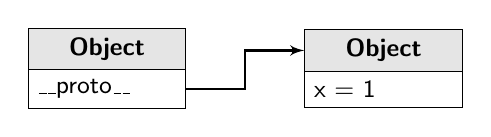
\begin{tikzpicture}[node distance=1.5cm]
    \node (object1)
          [object, rectangle split parts=2]
          {\nodepart{text}\textbf{Object}
           \nodepart{second}\_\_proto\_\_};
    \node (object2)
          [object, rectangle split parts=2, right=of object1]
          {\nodepart{text}\textbf{Object}
           \nodepart{second}x = 1};
    \renvoi{object1.second east}{object2.text west};
  \end{tikzpicture}
\end{center}

Functions are first-class objects and constructors are implemented as
functions. Using the \texttt{new} operator, a fresh object is
instantiated. The execution environment allocates a new object and
sets its prototype to the constructor's \texttt{prototype} property,
which is initially an empty object. If a property lookup on the
instance fails, the value of the constructor's \texttt{prototype}
property will be used instead. When a constructor is called
using \texttt{new}, the implicit variable \texttt{this} refers to the
instance is bound inside the body. This is also the case when a
function is called as a method, i.e., using property lookup in form of
\texttt{object.function()}, rather than
\texttt{function(object)}. This mechanism is illustrated in
Listing~\ref{lst:js-example}.

\begin{lstlisting}[label=lst:js-example,caption=Using prototypes in JavaScript]
function Person(name) {
  this.name = name;
}
Person.prototype.hello = function () {
  return "Hello, " + this.name + "!";
}
var john = new Person("John");
// john.__proto__ = Person.prototype
john.hello() // $\Rightarrow$ "Hello, John!"
\end{lstlisting}

This already resembles typical class-based object orientation when
assuming the constructor as a ``class''.  Single inheritance can be
implemented using \\
\lstinline{class.prototype.__proto__ = superclass.prototype}

In Ralph, the macro \texttt{define-class} produces a constructor.
Additionally an object containing all properties (cf. slots in Dylan
and CLOS) of the class is generated. Finally, a call to the
runtime function \texttt{\%make-class} is generated and these values
and the superclass are passed as arguments. This is demonstrated in
Listing~\ref{lst:define-class}.

\begin{lstlisting}[label=lst:define-class,
    caption=Code produced by macro \texttt{define-class},
    escapechar=!
]
(define-class <person> (<object>)
  name)
!{\color{black!40}\rule[0.2em]{\linewidth}{0.5pt}}!
(define <person>
        (%make-class <object>
                     (%object "name" #f)
                     (%method <person> ())))
\end{lstlisting}

At runtime, \texttt{\%make-class} will setup the inheritance
relationship by setting the prototype property as shown above, and
keeping a reference to the superclass. Also, the prototype of the
object containing all properties is set to that of the superclass, so
that looking up properties of the class will also return inherited
ones, most specific first. The definitions are shown in
Listing~\ref{lst:make-class/inherit}.

\begin{lstlisting}[label=lst:make-class/inherit,
    caption=Definitions of \texttt{\%make-class} and \texttt{\%inherit}
]
(define-function %inherit (class superclass)
  (set! (get class "%superclass")
        superclass)
  (set! (get class "prototype" "__proto__")
        (get superclass "prototype"))
  (set! (get class "%properties" "__proto__")
        (get superclass "%properties"))
  class)

(define-function %make-class
    (superclass properties constructor)
  (set! (get constructor "%properties")
        properties)
  (when superclass
    (%inherit constructor superclass))
  constructor)
\end{lstlisting}

Similar to Dylan, the method \texttt{make} will allocate an instance of
the passed class, and \texttt{initialize} will perform the actual
initialization of all properties. If no values are passed to
\texttt{make}, the default forms, stored as functions, are used
instead. Listing~\ref{lst:make/initialize} contains the definitions of
both functions.

\begin{lstlisting}[label=lst:make/initialize,
    caption=Definitions of \texttt{make} and \texttt{initialize}
]
(define-function make (type #rest arguments)
  (bind ((object (%native-call "new" type)))
    (apply initialize object arguments)
    object))

(define-function %initialize-property
    (object properties arguments property)
  (unless (has? (get <object> "prototype")
                property)
    (bind ((value
            (or (get arguments property)
                (bind ((value
                        (get properties
                             property)))
                  (when value
                    (value))))))
      (set! (get object property) value))))

(define-method initialize
    ((object <object>) #rest rest)
  (bind ((arguments (as-object rest)))
    (if-bind (properties
              (get (type object)
                   "%properties"))
      (do (curry %initialize-property
                 object properties
                 arguments)
          (object-properties
           properties inherited?: #t))))
  object)
\end{lstlisting}

Recently, means of defining properties were added to JavaScript,
including default values and access restrictions, using
\sloppy\mbox{\texttt{Object.defineProperty}}. The approach described
above was chosen, as this feature is not yet available in all
execution environments and its performance is poor compared to normal
functions which set and get properties.

\subsubsection{Functions}

There are two types of functions: methods and generic functions. A
generic function can contain one or more methods. Both generic
functions and methods consist of a typed argument list and
code. Similar to CLOS, functions are first-class citizens, and not
defined inside of classes. When a method is called, its body is
directly executed. When a generic function is called, the first argument
is compared to the typed argument lists of all defined methods of the
generic function and the most specific one is invoked. This is the
means of object-oriented (single) dispatch.

Dylan performs multiple dispatch, i.e., all arguments and all elements
of the argument lists are considered when determining the applicable
method. Ralph is currently limited to single dispatch, i.e., only the
first argument and first type of each argument list is taken into
consideration.

Similar to the implementations of the class hierarchy, this design
choice is due to the performance problems associated with naively
adopting this concept, i.e., adding methods to a generic function,
which performs multiple dispatch on each call. Not using the prototype
system has drastic performance implications, as usage like shown in
Listing~\ref{lst:js-example} is heavily optimized by execution
environments, e.g., by replacing call-sites with direct jumps.

The runtime of Ralph uses prototypes. The macro \texttt{define-method}
produces a call to the runtime function \texttt{\%make-method}, which
receives the method to be defined, along the name and type for which
it is specialized. At runtime, the function \texttt{\%make-method}
adds the method to the \texttt{prototype} property of the type. The
method is thus actually added to the class internally. If no generic
function exists yet, it is implicitly created. When the method is
called, the implicitly generated generic function performs the actual
dispatch: it looks up the method via its name in the object and
invokes it if it exists. This part is usually inlined by the execution
environment. Both definitions are shown in
Listing~\ref{lst:make-method} and Listing~\ref{lst:make-generic}.

\begin{lstlisting}[label=lst:make-method,
    caption=Definition of \texttt{\%make-method}
]
(define-function %make-method
    (name function setter? type existing)
  ;; definition
  (set! (get function "%name") name)
  (set! (get function "%setter?") setter?)
  (set! (get function "%type") type)
  (set! (get type "prototype" name) function)
  ;; implicit definition of generic function?
  (if (and existing
           (get existing "%generic?"))
      existing
      (%make-generic name))))
\end{lstlisting}

\begin{lstlisting}[label=lst:make-generic,
    caption=Definition of \texttt{\%make-generic}
]
(define-function %make-dispatcher (name)
  (method (object)
    (bind ((function
             (get (%native
                    "(" object "== null ?"
                    " false : " object ")")
                  name)))
      (%infix "&&"
              function
              ((get function "apply")
               object %all-arguments)))))

(define-function %make-generic (name)
  (bind ((dispatcher (%make-dispatcher name)))
    (set! (get dispatcher "%generic?") #t)
    (set! (get dispatcher "%name") name)
    dispatcher))
\end{lstlisting}

Inside the body of a method in Ralph, the implicit variable
\texttt{next-method} is a reference to the next most specific method.
It is a symbol macro (described in the next section) compiling to a
call to the runtime function \texttt{\%next-method}, passing the
current method. The implementation of \texttt{\%next-method} is shown
in Listing~\ref{lst:next-method}.

\begin{lstlisting}[
    caption=Determining the next most specific method,
    label=lst:next-method
]
(define-function %next-method (function)
  (bind ((name (get function "%name"))
         (proto (get function "%type"
                     "prototype"
                     "__proto__")))
    (get proto name)))
\end{lstlisting}

\pagebreak

An exemplary program demonstrating the use of classes and methods in
Ralph is shown in Listing~\ref{lst:classes-methods}.
Figure~\ref{fig:person-student} shows the internal object structure
after both classes are defined.

\begin{lstlisting}[
    caption=Using classes and methods in Ralph,
    label=lst:classes-methods
]
(define-class <person> (<object>)
  (name ""))

(define-method hello ((person <person>))
  (format-to-string "Hello, %s!"
                    (get person "name")))

(define-class <student> (<person>) id)

(define-method hello ((student <student>))
  (concatenate (next-method student)
               (format-to-string
                " Student #%d!"
                (get student "id"))))

(bind ((john (make <student> name: "John" id: 23)))
  (hello john))
;; $\Rightarrow$ "Hello, John! Student #23"
\end{lstlisting}

\vspace{2em}

\begin{figure}[H]
  \centering
  \caption{Structure after definition of classes <person> and
    <student>}
  \label{fig:person-student}
  \begin{tikzpicture}[node distance=1cm]
    \node (person)
          [object, rectangle split parts=3]
          {\nodepart{text}\textbf{Function} <person>
           \nodepart{second}prototype
           \nodepart{third}\%properties};
    \node (personProto)
          [object, rectangle split parts=2, right=of person, text width=3.5cm]
          {\nodepart{text}\textbf{Object}
           \nodepart{second}hello =
           \lstinline[breaklines]|function () { return "Hello, "  +  this.name + "!" }|};
    \node (personProps)
          [object, rectangle split parts=2, right=of person,
            below=0.5cm of personProto, text width=3.5cm]
          {\nodepart{text}\textbf{Object}
           \nodepart{second}name = \lstinline|function () { return "" }|};
    \node (student)
          [object, rectangle split parts=4, below=2.5cm of person]
          {\nodepart{text}\textbf{Function} <student>
           \nodepart{second}prototype
           \nodepart{third}\%properties
           \nodepart{fourth}\%superclass};
    \node (studentProto)
          [object, rectangle split parts=3, right=of student, text width=3.5cm]
          {\nodepart{text}\textbf{Object}
           \nodepart{second}hello = \lstinline|function () { $\ldots$ }|
           \nodepart{third}\_\_proto\_\_};
    \node (studentProps)
          [object, rectangle split parts=3, right=of student,
            below=0.5cm of studentProto, text width=3.5cm]
          {\nodepart{text}\textbf{Object}
           \nodepart{second}id = false
           \nodepart{third}\_\_proto\_\_};
    \renvoi{person.third east}{personProps.text west}
    \renvoi{person.second east}{personProto.text west}
    \renvoi{student.third east}{studentProps.text west}
    \renvoi{student.second east}{studentProto.text west}
    \renvoi[left=1em]{student.fourth west}{person.text west}
    \renvoi[right=1em]{studentProto.third east}
           {personProto.text east}
    \renvoi[right=2em]{studentProps.third east}
           {personProps.text east}
  \end{tikzpicture}
\end{figure}

\vspace{1em}

\subsection{Macro system}

\subsubsection{Definition and usage of Macros}

%% motivation/introduction

Macros were not part of the early specification of Dylan and the
standardized Dylan only features a macro-system based on
pattern-matching of code fragments and rewrite rule-based
transformation. We decided to implement a more powerful system,
allowing macro transformers to perform general computations.
\pagebreak

Similar to Dylan, Ralph performs hygienic expansion. We chose to adopt
the macro system of Clojure, which is a hygienic variant of the Common
Lisp macro system based on quasi-quotation. Definition and execution
of macro transformers, as well as approach to hygiene, substantially
differs from Dylan.

%% definition

Macro transformers can be defined using the \texttt{define-macro}
form. They are implemented as normal functions, but also registered as
macros when evaluated. Listing~\ref{lst:inc} contains a macro
definition of the increment operation \texttt{inc!}.

\begin{lstlisting}[caption=Macro definition of \texttt{inc!},label=lst:inc]
(define-macro inc! (object value)
  `(set! ,object
         (+ ,object ,(or value 1))))
\end{lstlisting}

In addition to normal quoting through \texttt{quote} or its reader
macro (the ``quote'' character \lstinline{'}), a form can be
syntax-quoted (using ``backquote'' \lstinline{`}). The expression that
follows is quoted, and in case it is a list, every subexpression is
quoted recursively as well. Quotation can be prevented using unquote
(the ``comma'' \lstinline{,} character) and spliced into the outer
expression using unquote-splicing (the ``comma'' and ``at'' characters
combined \lstinline{,@}). The behavior is similar to that of Common
Lisp's equivalents.

The major difference is syntax-quote, as in addition to quoting, it
also ``resolves'' symbols in the current module. If the symbol is
locally bound, either through a global definition or a local binding,
it is qualified with the current module. If it is not bound and
imported from another module, it is qualified with this
module. Otherwise the current module  will be used for
qualification. For all other forms, such as numbers, strings,
keywords, etc., syntax-quoting has the same effect as normal quoting,
i.e., \lstinline{`x} is equivalent to \lstinline{'x}.

\begin{aquote}{Rich Hickey, creator of Clojure}
  ``It is unique, and it is not renaming. I call the process resolving,
  and the basic purpose is hygiene - macros yield qualified symbols
  reflecting their meanings at macro definition time.''
\end{aquote}

Listing~\ref{lst:syntax-quote} shows an example demonstrating this
behavior and also how unqualified symbols can be introduced by
unquoting a symbol. Through the use of syntax-quote, macros are
therefore producing qualified symbols.

\begin{lstlisting}[
    label=lst:syntax-quote,
    caption={Example of using syntax-quote in module \texttt{bar},
      importing \texttt{x} and \texttt{y} from \texttt{foo}}
]
(bind ((x 23))
  `(y x ,x ,'x))
;; $\Rightarrow$ (foo::y bar::x 23 x)
\end{lstlisting}

The second difference of this approach to hygiene is in the expansion
pass. Both \texttt{define} and \texttt{bind} prevent the binding of
qualified symbols. In connection with macros producing qualified
symbols by default, this ultimately prevents unintentional capturing
of variables and qualified symbols cannot be bound to other values.
Still, hygiene can be intentionally broken by introducing an
unqualified symbol as shown before. Listing~\ref{lst:expansion}
illustrates this behavior.

\begin{mylisting}[h]
  \caption{Behavior of macroexpansion}
  \label{lst:expansion}
  \vspace{-2em}
  \begin{sublisting}{Macro definition producing an error at expansion
      time, caused by binding qualified symbol \texttt{x}}
    \begin{minipage}[b]{.7\textwidth}
      \begin{lstlisting}
(define-macro foo ()
  `(bind ((x $\ldots$))
     $\ldots$))
      \end{lstlisting}
    \end{minipage}
  \end{sublisting}
  \hfill
  \begin{sublisting}{Intentional breaking of hygiene by binding an unqualified symbol}
    \begin{minipage}[b]{.7\textwidth}
      \begin{lstlisting}
(define-macro foo ()
  `(bind ((,'x $\ldots$))
     $\ldots$))
      \end{lstlisting}
    \end{minipage}
  \end{sublisting}
\end{mylisting}
\vspace{-0.5em}

As shown in Listing~\ref{lst:inc-example}, the macro definition and
use of \texttt{inc!} defined in Listing~\ref{lst:inc} is therefore
safe. Rebinding \texttt{+} before using the macro does not lead to
problems, because the expansion is referring to \texttt{ralph/core::+}.

\begin{lstlisting}[caption=Use of macro \texttt{inc!},label=lst:inc-example]
(bind ((x 1)
       (+ -))
  (inc! x)
  x)
;; $\Rightarrow$ 2
\end{lstlisting}

The macro system also supports symbol macros. While normal macro calls
look like function calls, symbol-macro calls look like symbols. They
can be defined using \texttt{define-symbol-macro}.

\subsubsection{Phase separation}

Procedural macros need phase separation \cite{flatt2002}, i.e.,
distinguishing between run-time and compile-time evaluation of code,
as macros will likely refer to other definitions. Most Lisp
dialects require the programmer to follow certain protocols when
defining macros and explicitly state the phase in which the code
should be evaluated. For example, Common Lisp provides the special
operator \texttt{eval-when}, Scheme a reflective tower involving the
primitive forms \texttt{begin-for-syntax}, \texttt{define-for-syntax},
etc. Some macro systems are more sophisticated and perform inference
based on usage. Listing~\ref{lst:eval-when} shows an example written
in Common Lisp. The \texttt{eval-when} form is necessary to instruct
the compiler to run the function definition of \texttt{transform}
during compilation.

\begin{lstlisting}[
    label=lst:eval-when,
    caption=Usage of \texttt{eval-when} in Common Lisp
]
  (eval-when (:compile-toplevel :execute
              :load-top-level)
    (defun transform (form)
      $\ldots$))

 (defmacro foo (form)
   (transform form))

 (foo $\ldots$)
\end{lstlisting}

Providing such a macro system increases the complexity of a compiler
implementation drastically and is even more complicated when a module
system is involved. Ralph does not allow a call to a macro from within
the module where the macro is defined. This means that all code of a
module is run in the same compilation phase and it is not possible for
the programmer to interleave different phases.

To use a macro in a module, its definition needs to be inside another
module. Like importing definitions for run-time through the
\texttt{import} keyword parameter of the \texttt{define-module} form,
definitions can be imported for compile-time use through the
\texttt{compile-time-import} keyword parameter (cf. Scheme's
\texttt{require-for-syntax}). When the module using the macro is
compiled, the compiler will first compile the compile-time imported
modules and load them. As described, macros are just functions and
thus they are available after loading the module defining them.
Listing~\ref{lst:full-macro-example} contains a full example
demonstrating the definition and usage of macros in Ralph.

\begin{mylisting}[h]
  \caption{Final example of defining and using macro \texttt{inc!}}
  \label{lst:full-macro-example}
  \vspace{-2em}
  \begin{sublisting}{Module \texttt{example}: Use of macro \texttt{inc!}}
    \begin{minipage}[b]{.7\textwidth}
      \begin{lstlisting}
(define-module example
  import: (ralph/format)
  compile-time-import:
    (example-macros))

(bind ((x 1)
       (+ -))
  (inc! x)
  (format-out "%d" x))
      \end{lstlisting}
    \end{minipage}
  \end{sublisting}
  \hfill
  \begin{sublisting}{Module \texttt{example-macros}: Definition of macro \texttt{inc!}}
    \begin{minipage}[b]{.7\textwidth}
      \begin{lstlisting}
(define-module example-macros
  export: (inc!))

(define-macro inc! (object value)
  `(set! ,object
         (+ ,object ,(or value))))
      \end{lstlisting}
    \end{minipage}
  \end{sublisting}
\end{mylisting}
\vspace{-0.5em}

The first pass of the compilation does a full macro-expansion, which
expands each expression of the program into a minimal IR. When
encountering a \texttt{define-module}, all modules referred to by the
\texttt{compile-time-import} keyword are compiled and
loaded. Evaluating the module will bind possible macros as previously
discussed. The macroexpansion pass also resolves all remaining symbols
that have not already been resolved through syntax quoting, so that
the following passes are working on a program where all symbols
are already fully qualified.

Both the hygienic macro system and simplified phase separation are
easy to implement, and powerful enough to write sophisticated macros.
The only burden on the programmer is to separate macros in a different
module, but is also less error-prone.

\subsection{Free variables}

Following the macroexpansion pass, all \texttt{define} forms are
transformed to assignments. For every unique identifier that is
defined, an appropriate variable declaration (\texttt{\%define})
is prepended to the program. As the macro transformers might have
introduced new identifiers, the program is analyzed for free
variables. For every free variable, a variable declaration is added.
This is also important, to allow the usage of definitions that
are still to be defined later in the program.

Even though the free variables are qualified symbols, they might refer
to imported definitions. Hence, for symbols referring to imported
definitions and for external references, appropriate internal import
code is generated, which can be considered as ``linking''.

\subsection{Scoping}

Ralph's \texttt{bind} macro (cf. Common Lisp special operator
\texttt{let*}) allows sequential binding. Bindings can also be
introduced using \texttt{method} (cf. Common Lisp special operator
\texttt{lambda}). For example, the forms in Listing~\ref{lst:bindings}
are both creating $n$ bindings and are thus equivalent. Many compilers
targeting JavaScript naively perform the translation from (a) to (b)
and generate $n$ closures. Closures are expensive in JavaScript,
thus this has a high impact on performance.

\begin{mylisting}[h]
  \caption{Introducing bindings}
  \label{lst:bindings}
  \vspace{-2em}
  \begin{sublisting}{Binding using \texttt{bind}}
    \begin{minipage}[b]{.42\textwidth}
      \begin{lstlisting}
(bind ((x1 y1)
       $\ldots$
       (xn yn))
  (f x1 $\ldots$ xn))
      \end{lstlisting}
    \end{minipage}
  \end{sublisting}
  \hfill
  \begin{sublisting}{Binding using \texttt{method}}
    \begin{minipage}[b]{.48\textwidth}
      \begin{lstlisting}
((method (x1)
    $\ldots$
    ((method (xn)
       (f x1 $\ldots$ xn))
     yn)
    $\ldots$)
 y1)
      \end{lstlisting}
    \end{minipage}
  \end{sublisting}
\end{mylisting}
\vspace{-0.5em}

An alternative is using the statement \sloppy\mbox{\texttt{with
    (\textit{object}) \textit{statement}}}, which introduces a new
lexical environment. For all name lookups inside the given statement,
the object's properties are examined. This dynamic feature can not be
trivially optimized and commonly results in bad performance in
execution environments. It also has been deprecated in the latest
version of JavaScript and therefore is not a viable option.

Ralph performs $\alpha$-conversion to solve this problem, which
renames identifiers introduced through definitions and bindings to
fresh names. Thus, Ralph does not need to introduce anonymous functions
which are immediately invoked for binding. This also solves the
previously described hoisting problem. A nested binding with equal
variable names is transformed into an expression using the internal
single-expression bind macro \texttt{\%bind} and renaming is
performed, making variables distinctive.
Listing~\ref{lst:alpha-conversion} contains an example.

\begin{lstlisting}[label=lst:alpha-conversion,
    caption=Expansion and alpha-conversion,escapechar=!
]
(bind ((x (bind ((x 1)) x))) x)
!{\color{black!40}\rule[0.2em]{\linewidth}{0.5pt}}!
(%bind (x1 (%bind (x2 1) x2)) x1)
\end{lstlisting}

\subsection{Code generation}

Many compilers targeting JavaScript use a direct-style representation
and perform naive code generation, i.e., the representation of the
original program is used and is not further transformed into another
form. As described before, this is easier to implement, but produces
less optimal code.

JavaScript specifies both statements and expressions and for most
forms, both versions exists. For example, the conditional exists as
the \texttt{if} statement and as an expression in form of the ternary
operator \texttt{?:}. In both branches of the \texttt{if} statement
further statements can appear, but in the operator only expressions
are valid.


Naive code generators have to emit the correct form, depending on the
current context. For instance, inside the body of a function,
statements are allowed. For a binding form, variable declarations are
generated, their value being an expression. For a conditional an
expression can be generated. In case the value is a form for which no
equivalent expression exists, the compiler needs to wrap the
statements inside an anonymous function that is immediately
invoked. This example is shown in Listing~\ref{lst:wrappers}. As a
result, excessive amounts of closures need to be generated,
resulting in poor performance in current execution environments.

\begin{mylisting}[h]
  \caption{Naive code generation}
  \label{lst:wrappers}
  \vspace{-2em}
  \begin{sublisting}{Generation of \texttt{if} expression}
    \begin{minipage}[b]{.44\textwidth}
      \begin{lstlisting}[escapechar=!]
(bind
  ((x1 (if x 1 2)))
  $\ldots$
!{\color{black!40}\rule[0.2em]{\linewidth}{0.5pt}}!
var x1 = x ? 1 : 2;
  $\ldots$
      \end{lstlisting}
    \end{minipage}
  \end{sublisting}
  \hfill
  \begin{sublisting}{Generation of nested binding}
    \begin{minipage}[b]{.45\textwidth}
      \begin{lstlisting}[escapechar=!]
(bind
  ((x1 (bind ((x2 1))
         (+ x2 1))))
  $\ldots$
!{\color{black!40}\rule[0.2em]{\linewidth}{0.5pt}}!
var x1 =
  (function () {
    var x2 = 1;
    return x2 + 1;
  })();
$\ldots$
      \end{lstlisting}
    \end{minipage}
  \end{sublisting}
\end{mylisting}
\vspace{-0.5em}

More sophisticated compilers translate the program into an IR and
perform further transformations and optimizations on it. A common IR
is continuation passing style \cite{sussman75scheme} (CPS), where each
function has an additional parameter, which is a continuation
containing the remaining program. The last statement in each function
is a call to this continuation with the computed result. CPS is
well suited for optimization techniques \cite{kennedy2007}.

As every call in CPS is a tail-call, using the program without tail
call optimization (TCO) will grow both the constructed continuation
and the call stack. However, JavaScript and most commonly used target
languages (e.g. C, Java) provide no guarantees about tail-call
optimization. Hence, using a program in CPS form for code generation
is not suitable: it will have poor performance compared to a
traditional return-based calling convention and impairs
interoperability. It would be necessary to translate the program back
to direct style, requiring yet another translation pass, implementing
a sophisticated algorithm to handle continuations using exceptions
(cf. scheme2js \cite{loitsch2009scm2js}), or translating it further
into a low level instruction set and implementing a custom stack in
JavaScript (cf. Gambit-JS \cite{thivierge2012}).

The approach used in Ralph's compiler builds on the idea of using a
direct-style approach like naive compilers instead. Ralph produces
code similar to hand-written one, delivering better performance and
readability. The main performance improvement over naive compilers is
the reduced amount of generated closures. Considering that all forms
in JavaScript are available as statements, but only a subset as
expressions, it is appropriate to always generate statements, instead
of generating code depending on context and producing additional
closures.

A perfect match is the administrative normal form \cite{flanagan1993}
(ANF), which requires that all arguments of a function call to be
trivial (meaning constants, variables or functions) and non-trivial
argument computations to be captured through bindings.
Listing~\ref{lst:anf-example} shows that this definition solves cases
such as nested bindings, eliminating the production of closures.

\begin{lstlisting}[
    label=lst:anf-example,
    caption=Transformation to ANF,
    escapechar=!
]
(bind ((x (+ (bind ((y 1))
               (+ y 2))
             3)))
  (+ (- x 4) x))
!{\color{black!40}\rule[0.2em]{\linewidth}{0.5pt}}!
(%bind (y 1)
  (%bind (g1 (+ y 2))
    (%bind (x (+ g1 3))
      (%bind (g2 (- x 4))
        (+ g2 x)))))
\end{lstlisting}

However, it is apparent that many bindings are generated, which
increases the number of lookups in the lexical environment. The number
of generated redexes can be reduced by adjusting the definition of
triviality. Expressions for which no JavaScript statements are
produced are also considered trivial and are not lifted. Expressions
that do generate statements and still need to be lifted are expression
sequencing (\texttt{\%begin}), conditionals (\texttt{\%if}), loops
(\texttt{\%while}), bindings (\texttt{\%bind}) and exception handling
(\texttt{\%try}). Assignments (\texttt{\%set}) whose values do not
generate statements, and function calls whose arguments do not
generate statements will not generate statements and need not to be
lifted. This new definition of triviality is determined by the
predicate \texttt{generates-statements?} shown in
Listing~\ref{lst:generates-statements}.

\begin{lstlisting}[label=lst:generates-statements,
    caption=Determining generation of JavaScript statements]
(define-function generates-statements? (form)
  (if (and (instance? form <array>)
           (not (empty? form)))
      (select (symbol-name (first form)) ==
        (("%begin" "%if" "%while"
          "%bind" "%try")
         #t)
        (("%set")
         (generates-statements? (last form)))
        (("%method") #f)
        (else:
         (any? generates-statements? form)))
      #f))
\end{lstlisting}

As a result, the example can now be reduced as shown in
Listing~\ref{lst:anf-example2}.

\begin{lstlisting}[label=lst:anf-example2,
    caption=Resulting IR when using adjusted ANF]
(%bind (y 1)
  (%bind (g1 (+ y 2))
    (%bind (x (+ g1 3))
  (+ (- x 4) x))))
\end{lstlisting}

The adjusted version also needs to take the evaluation order into
account. If any subexpression needs to be lifted, at least all
subexpressions occuring before it need to be lifted as well, even if
they are considered trivial. This is demonstrated in
Listing~\ref{lst:evaluation-order}.


\begin{lstlisting}[label=lst:evaluation-order,
    escapechar=!,
    caption=Adjusted ANF preserves evaluation order]
(+ (+ 2 2)
   (bind ((x 1))
     (f x)))
!{\color{black!40}\rule[0.2em]{\linewidth}{0.5pt}}!
(%bind (g1 (+ 2 2))
  (%bind (x 1)
    (%bind (g2 (f x))
      (+ g1 g2))))
\end{lstlisting}

After the transformation to ANF, the code is further transformed to
``statement'' form, resembling the specifics of JavaScript, by adding
explicit return statements to method bodies. In ANF, bindings may
still have values which may produce statements in JavaScript. If a
value of a binding is control-flow (if, while, etc.), it is moved
to the body and explicit assignments are added to the value. Finally,
bindings are flattened to variable declarations and possibly combined.
Nested expression sequencing are flattened as well. An example is
presented in Listing~\ref{lst:statements/flattening}, showing ANF,
statement transformation/flattening, and final JavaScript.

\begin{lstlisting}[escapechar=!,
    label=lst:statements/flattening,
    caption=\sloppy\mbox{Transformation to statements and flattening}
]
(%bind (x1 (%if $\ldots$
                (%bind (x2 $\ldots$)
                  $\ldots$
                  (foo x2))
                3))
!{\color{black!40}\rule[0.2em]{\linewidth}{0.5pt}}!
(%begin
  (%var (x1 #f))
  (%if $\ldots$
       (%begin
         (%var (x2 $\ldots$))
         $\ldots$
         (%set x1 (foo x2)))
       (%set x1 3))
!{\color{black!40}\rule[0.2em]{\linewidth}{0.5pt}}!
var x1;
if ($\ldots$) {
  var x2 = $\ldots$;
  $\ldots$
  x1 = foo(x2);
} else
  x1 = 3;
\end{lstlisting}

%% TODO: also show intermediate step?
%% (%bind (x1 #f)
%%   (%if $\ldots$
%%        (%bind (x2 $\ldots$)
%%          $\ldots$
%%          (%set x1 (foo x2)))
%%        (%set x1 3))
%%   $\ldots$

%% TODO: show resulting JS?

\subsection{Truth}

Lisp dialects differ in the notion of truth. In Common Lisp, the
single value \texttt{nil} is equivalent to the empty list and used to
represent the false value. Non-\texttt{nil} values are treated as
true. Dylan is using the same notion as Scheme: the values
\texttt{\#t} and \texttt{\#f} represent truth and falsity respectively.
Every non-\texttt{\#f} value is treated as true, even the empty list.

In JavaScript, the values \texttt{false}, \texttt{undefined},
\texttt{null}, \texttt{+0}, \texttt{-0}, \texttt{NaN}, and the empty
string are treated as false. To provide consistency in Ralph,
\texttt{\#f} is mapped to \texttt{false} and is the only false value
available to programmers. Internally, only the values \texttt{false},
\texttt{undefined} and \texttt{null} are treated as false. The
function \texttt{isTrue} as shown in Listing~\ref{lst:isTrue}
implements this behavior.

\begin{lstlisting}[label=lst:isTrue,caption=Determining truth]
function isTrue(value) {
  return (value != null)
         && (value !== false);
}
\end{lstlisting}

To implement these semantics in conditionals, the values of the tests
in \texttt{\%if} and \texttt{\%while} expressions are wrapped in a
call to \texttt{isTrue}. To treat all false values as instances of
\texttt{Boolean}, the definition of \texttt{isInstance} as shown in
Listing~\ref{lst:isInstance} is used. Generic function dispatch is
also safe for the values \texttt{undefined} and \texttt{null}. In
general, treating \texttt{null} and \texttt{undefined} as false leads
to less exceptions at runtime.

\begin{lstlisting}[label=lst:isInstance,caption=Determining if
    \texttt{object} is an instance of \texttt{type}]
function isInstance (object, type) {
  return isTrue(object) ?
      ((object instanceof type) ||
       (object.constructor === type))
      : (type === Boolean);
}
\end{lstlisting}


The identity and equality problems common in JavaScript are solved by
providing the functions \texttt{==} for identity and \texttt{=} for
equality. Both take one or more arguments and iteratively invoke their
binary counterparts \texttt{binary==} and \texttt{binary=}. The binary
identity function is simply mapped to the JavaScript identity operator
\texttt{===}. The binary equality function is generic. Equality
methods for built-in types are provided and can also be added by
the programmer by defining a method for \texttt{binary=}.

\subsection{Optimizations}

By using the compilation approach as outlined, Ralph's compiler
is already producing fast code for the high-level features of the
language. This is accomplished using an appropriate IR and therefore
generating code that is similar to hand-written, imperative code,
which execution environments are able to optimize fairly well.

Ralph's compiler applies several optimizations to improve the
performance of the generated code even further. Minimizing the code
size is not important, as there are many existing tools to reduce the
size of JavaScript. Some other compilers rely solely on
post-processing tools and source-to-source compilers to perform
further optimizations. Often, optimizing code requires high-level
information, which are missing in the output or cannot necessarily be
expressed appropriately (cf. ClojureScript).

In general, generated code and code in the runtime is optimized so it
performs well on all execution environments, i.e., the compiler does
not target or prefer a specific JavaScript engine. Another problem is
compatibility. Only features available in all commonly used
execution environments are used. The optimizations applied when
compiling from a high-level language to another differ from the
optimizations usually applied by compilers targeting low-level code.

Even though most JavaScript engines try to inline code automatically,
i.e., replace a call site with the body of the called function,
performing manual inline expansion ensures this happens for all
engines where known, and can yield great performance gains. For this
purpose, the macro \texttt{define-module} also accepts an
\texttt{inline} keyword, taking a list of definitions that should be
inlined. The programmer is thus able to provide hints to the
compiler. This feature is especially useful, as in many occasions only
``wrapper'' functions are created, that actually only call built-in
functions. For example, the standard function \texttt{push-last} is
actually calling \texttt{Array.prototype.push} on the array. The
definition is shown in Listing~\ref{lst:push-last}. By inlining
definitions, the compiler can also apply further optimizations.

\begin{lstlisting}[label=lst:push-last,caption=Definition of standard
    function \texttt{push-last}]
(define-function push-last (array value)
  (%native array ".push(" value ")")
  array)
\end{lstlisting}

Normally symbols are compiled to a call to the interning function,
which either returns the symbol instance if it already exists, or
creates and returns a new instance. The compiler lifts the calls to
the top-level, creates only one binding and call for each individual
symbol, and uses the binding for all remaining occurrences.

The Ralph compiler also reduces property access where possible. For
example, it is common for libraries written in JavaScript to expose
functionality by providing an object containing all ``exported''
definitions. Programs written in JavaScript usually perform
repeated property access on this object. When importing definitions
from other modules, the compiler only creates one binding for the
access to the definition. The binding is used for all subsequent
references.

Ralph features many imperative primitives, such as iteration over
collections through the macro \texttt{for-each} and loops using the
macros \texttt{while} and \texttt{for}. However, recursion is also
commonly used in functional languages such as Lisp and as discussed,
might grow the stack. Most compilers targeting lower-level languages
like C, can use optimizations techniques such as allocating call
frames on the heap (``Cheney on the M.T.A.'' \cite{baker1995}). This
method can only be used when emulating low-level instructions
(cf. Gambit-JS), but is not applicable when generating high-level
JavaScript.  Ralph's compiler performs simple tail-call optimization:
simple tail-recursion is eliminated by a transformation to a loop.

\section{Limitations}\label{sec:limitations}

Due to limitations imposed by the JavaScript language and its
implementations, Ralph makes certain trade-offs which features of
Dylan are supported. Unlike Dylan, Ralph only supports single
inheritance and single dispatch, to make use of the fast built-in
prototype-based object-system: The majority of applications written in
JavaScript tend to use a single inheritance, single dispatch
class-based object-system based on prototypes. JavaScript engines
heavily optimize for this use-case. For example, the V8 engine creates
hidden classes for objects\footnote{See
  \url{http://developers.google.com/v8/design}},
based on earlier work in Self \cite{chambers1989}.

Non-local returns could be represented through exceptions, but tests
have shown such an approach has a large impact on performance too, as
the implementation of exceptions in current environments is very
slow. For instance, V8 is currently not optimizing any functions that
contain \texttt{try}/\texttt{catch} statements. Exceptions could have
also been used to implement dynamic variables.

\vspace{-0.3em}
Multiple return values are not supported. This feature can be
implemented by using the implicit \texttt{arguments} object, available
inside the body of a function, that contains all arguments passed to the
function. Its property \texttt{callee} refers to the called function.
Further, its \texttt{caller} property refers to the calling function.
This allows passing arbitrary values back to the call-site.
However, it has a large performance impact and its use is deprecated.

\vspace{-0.3em}
Ralph also only exposes JavaScript's exception handling to the
programmer and does not provide a full condition system that does
stack unwinding protection. As a result, Ralph does not support
restarts.


\section{Further Work and Conclusion}\label{sec:future}

The compiler of Ralph is already self-hosting, i.e. it is written in
Ralph and is able to compile itself. It is currently in its third
iteration and we plan to extend the current implementation with
support for multiple inheritance and multiple dispatch. We want to
look into further optimization using partial dispatch
\cite{bachrach99}.

\vspace{-0.3em}
We plan to implement more optimizations (e.g. constant folding,
dead-code elimination, etc.) to improve the performance of generated
code. The compiler is also not performing any static type checking and
type inference yet, which could provide warnings of possible bugs to
the programmer and used for further optimization. For example,
currently a call to \texttt{isTrue} is inserted into all conditionals,
even though it might not be required, e.g., if it can be statically
determined that the value is of type boolean. To improve the safety
of the language, immutable data structures could be provided, similar
to Clojure/ClojureScript. It is also desirable to employ more
sophisticated tail-call elimination, e.g., to handle mutual
tail-recursion.

\vspace{-0.3em}
The IR of the final pass of compilation targets a language that
supports high-level features, such as closures, first-class functions
and garbage collection. Possible candidates for further backends could
be other scripting languages. For example, Lua has a dynamic nature
and semantics very similar to JavaScript. Another interesting
language is Objective-C, especially when considering its increasing
usage on mobile devices. Its latest version added support for closures
and automatic memory management.

\vspace{-0.3em}
We showed in this paper the common problems encountered when
developing applications in JavaScript and presented the Lisp dialect
Ralph as a practical solution. We showed that it is feasible to design
and implement a compiler that generates efficient JavaScript, by
making design trade-offs and utilizing a compilation approach
based on the ANF. This is an alternative to popular approaches (naive,
CPS) and performs well. Ralph has  been already successfully used to
implement a fairly large user-interface library\footnote{Available at
  \url{https://github.com/turbolent/ui}} for HTML5.

Many thanks to Hannes Mehnert for valuable advice, feedback on this
paper and wording improvements.

\bibliographystyle{abbrv}
\bibliography{paper}

\end{document}
